\documentclass[border=3pt,tikz]{standalone}
% Shared look for every TikZ figure in these notes.
% Included by each standalone figure file; also keeps the figures consistent
% with the colours used in the PDF and on the website.

\usepackage{tikz}
\usepackage{pgfplots}
\pgfplotsset{compat=1.18}
\usetikzlibrary{arrows.meta, decorations.markings, decorations.pathmorphing,
                patterns, calc, positioning}
\usepackage{amsmath}

% Series colours are the three validated categorical slots also used by the
% interactive widgets, so a path drawn in the printed notes and the same path on
% the website are the same colour. They clear the colour-vision-deficiency and
% contrast checks as a set; every path is direct-labelled as well, so colour is
% never the only thing carrying identity.
\definecolor{duPurple}{HTML}{68246D}
\definecolor{duBlue}{HTML}{2A78D6}
\definecolor{duRed}{HTML}{EB6834}
\definecolor{duGreen}{HTML}{1BAF7A}
\definecolor{duGrey}{HTML}{6B6B6B}

\tikzset{
  axisline/.style   = {-{Stealth[length=3mm]}, line width=0.7pt, black},
  path1/.style      = {duBlue,   line width=1.1pt},
  path2/.style      = {duRed,    line width=1.1pt},
  path3/.style      = {duGreen,  line width=1.1pt},
  statedot/.style   = {circle, fill=black, inner sep=1.4pt},
  arrowhead/.style  = {decoration={markings,
                        mark=at position #1 with {\arrow{Stealth[length=2.6mm]}}},
                       postaction={decorate}},
  lbl/.style        = {font=\small},
  slbl/.style       = {font=\footnotesize, duGrey},
  workfill/.style   = {duPurple, opacity=0.16},
}

\begin{document}
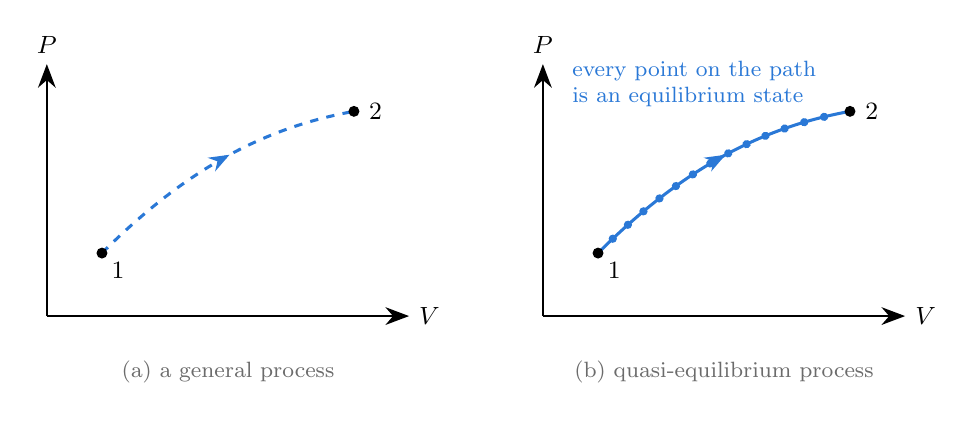
\begin{tikzpicture}
% (a) a general process: only the end states are equilibrium states
\begin{scope}
  \draw[axisline] (0,0) -- (4.6,0) node[right, lbl] {$V$};
  \draw[axisline] (0,0) -- (0,3.2) node[above, lbl] {$P$};
  \draw[path1, dashed, arrowhead=0.55] (0.7,0.8) .. controls (1.8,1.9) and (2.8,2.4) .. (3.9,2.6);
  \node[statedot] at (0.7,0.8) {}; \node[lbl, below right=0pt] at (0.7,0.8) {1};
  \node[statedot] at (3.9,2.6) {}; \node[lbl, right=2pt] at (3.9,2.6) {2};
  \node[slbl, below] at (2.3,-0.45) {(a) a general process};
\end{scope}
% (b) quasi-equilibrium: a continuous series of equilibrium states
\begin{scope}[shift={(6.3,0)}]
  \draw[axisline] (0,0) -- (4.6,0) node[right, lbl] {$V$};
  \draw[axisline] (0,0) -- (0,3.2) node[above, lbl] {$P$};
  \draw[path1, arrowhead=0.55] (0.7,0.8) .. controls (1.8,1.9) and (2.8,2.4) .. (3.9,2.6);
  \draw[draw=none, decoration={markings,
      mark=between positions 0.07 and 0.95 step 0.07 with {\fill[duBlue] (0,0) circle (1.5pt);}},
      postaction={decorate}]
    (0.7,0.8) .. controls (1.8,1.9) and (2.8,2.4) .. (3.9,2.6);
  \node[statedot] at (0.7,0.8) {}; \node[lbl, below right=0pt] at (0.7,0.8) {1};
  \node[statedot] at (3.9,2.6) {}; \node[lbl, right=2pt] at (3.9,2.6) {2};
  \node[slbl, below] at (2.3,-0.45) {(b) quasi-equilibrium process};
  \node[slbl, duBlue, align=left, anchor=west] at (0.25,2.95) {every point on the path\\is an equilibrium state};
\end{scope}
\end{tikzpicture}
\end{document}
